\documentclass[11pt]{article}
\usepackage[margin=1in]{geometry}
\usepackage{booktabs,tabularx,hyperref,graphicx,amsmath}
\title{Original VERA: CPU-Only Temporal-Position Audit}
\author{Research report for Shrid Pant}\date{October 27, 2026}
\begin{document}\maketitle
\textbf{Decision: fail the predeclared gate; stop further compute in this direction.} This is a retrospective score-stage audit, not a new detector or an end-to-end test of edited videos. No model weights, guiding questions or explanations were trained. GPU/model calls: zero.

\section{Measured result and agreed success criteria}
With unchanged detector evidence, original position weighting produces pooled ROC-AUC from 82.879\% to 86.607\% across five fixed shifts, a spread of 3.728 percentage points. Omitting the final weighting gives 85.600\% at every shift. Its worst-position benefit is 2.721 points, with paired whole-video bootstrap 95\% interval [1.307, 4.371]. Its original-order AUC cost is 1.007 points.

\begin{center}\small\begin{tabular}{lrrrrr}\toprule
Shift & Original AUC & No-pos AUC & Prior AUC & Original AP & No-pos AP\\\midrule
0\% & 86.607 & 85.600 & 61.799 & 32.745 & 28.717\\
20\% & 84.636 & 85.600 & 48.624 & 26.809 & 28.717\\
40\% & 82.879 & 85.600 & 37.551 & 22.187 & 28.717\\
60\% & 84.227 & 85.600 & 43.645 & 25.547 & 28.717\\
80\% & 86.036 & 85.600 & 58.335 & 33.377 & 28.717\\
\bottomrule\end{tabular}
\end{center}
All AUC/AP entries are percentages. AP means average precision, not trapezoidal precision--recall area. The prior-only diagnostic uses position without detector scores; it is not proposed as an anomaly detector.

\begin{center}\begin{tabularx}{\linewidth}{Xll}\toprule
Predeclared requirement & Observed & Pass\\\midrule
Original AUC spread at least 3pp & 3.728pp & yes\\
Worst-position benefit at least 3pp & 2.721pp & no\\
Paired 95\% interval lower bound above 0 & 1.307pp & yes\\
Original-order cost at most 1.5pp & 1.007pp & yes\\\bottomrule
\end{tabularx}\end{center}

All requirements must pass, including the five-video endpoint sensitivity. A positive confidence interval alone does not override the practical 3point threshold. There is measurable positional dependence, but the practical-benefit gate is not met. The result is not evidence of no effect; it is insufficient for the agreed resource-allocation criterion.

\begin{figure}[ht]\centering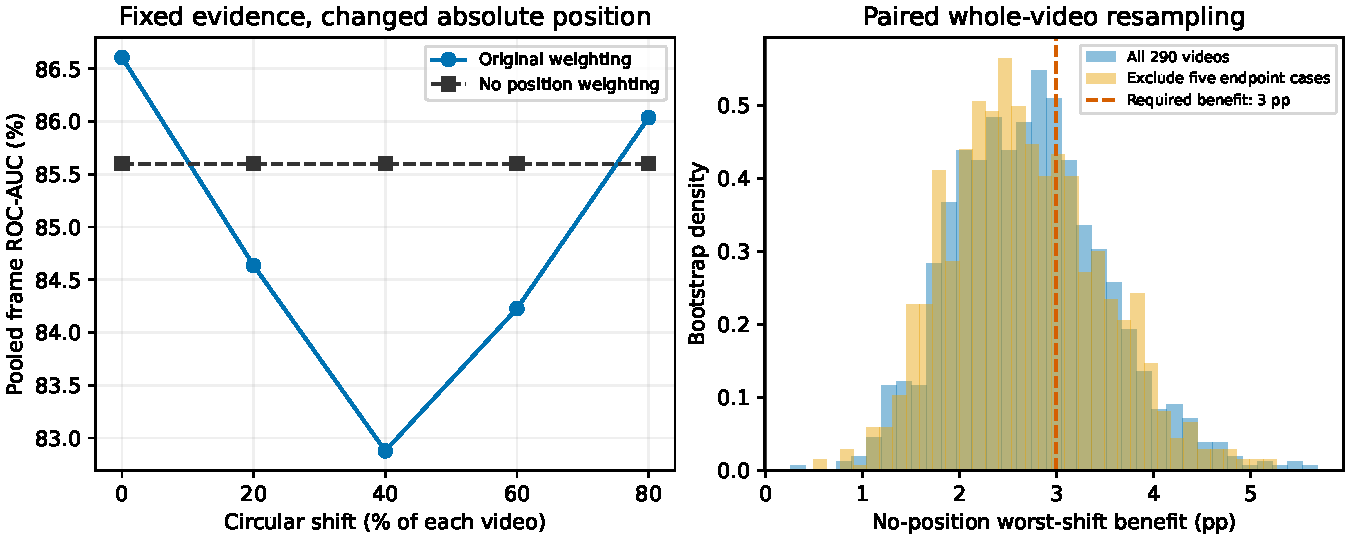
\includegraphics[width=\linewidth]{figures/position_audit.pdf}
\caption{Primary released-code retrieval ratio15\%. Left: same pre-position score/label pairs under five circular offsets. Right: paired whole-video bootstrap uncertainty for worst-position benefit. Dashed3pp line is the predeclared practical-benefit requirement.}
\end{figure}

\section{Sensitivity checks}
\begin{center}\small\begin{tabular}{lrrrrl}\toprule
Cohort & Spread & Benefit & 95\% CI & Cost & Pass\\\midrule
15 pct / 290 & 3.728 & 2.721 & [1.307, 4.371] & 1.007 & no\\
15 pct / 285 & 3.800 & 2.699 & [1.346, 4.374] & 1.100 & no\\
10 pct / 290 & 3.825 & 2.758 & [1.348, 4.388] & 1.067 & no\\
10 pct / 285 & 3.906 & 2.734 & [1.377, 4.362] & 1.173 & no\\
\bottomrule\end{tabular}
\end{center}
Spread, benefit, interval and cost are percentage points. Each cohort uses 1,000 paired whole-video resamples with seed 20261027. Five endpoint cases are Arson011, Arson016, Explosion033, Fighting003 and Shooting015. Their supplied interval ends exceed the recorded length by 1--2frames. Originals are preserved; primary labels follow upstream half-open slicing/clipping. Excluding these cases tests sensitivity without inventing new labels.

The released scoring script retrieves 15\% of segments, whereas VERA's paper describes 10\% for UCF. Primary implementation and the 10\% sensitivity were both frozen before measuring performance. We do not choose the better ratio after seeing outcomes. The paper reports86.55\% AUC; our unmodified released-code baseline is86.607\%, a difference of0.057 points, which is reported rather than tuned away. The predeclared10\% sensitivity baseline is86.548\%, which rounds to the published86.55\%.

\section{Inputs and exact reconstruction}
The official UCF archive contains 290 video IDs and 69,634 segment anchors, with no missing IDs or anchor-grid discrepancies. Existing labels contain 140 anomalous and 150 normal videos, spanning 1,111,808 frames. Author scores are reference outputs, not fresh VLM predictions. Previously consulted test sources make this a retrospective audit, not an untouched confirmation set.

The feature archive has 309,807,835 bytes and SHA256 \texttt{6b3e0a17091524c1635b68f18f8b1c5daaf067192d194e27d39de758db5f29e4}. All 290 feature members passed ZIP CRC, 1,024-dimension, row alignment, finiteness and nonzero-norm checks. RoadAccidents127 independently matches the feature checksum verified previously. Archive hashes record downloaded bytes; they are not an independently published authenticity proof. Files stay outside Git, with member and array hashes versioned.

The unmodified upstream \texttt{compute\_auc.py}, SHA256 \texttt{21e9705da3e8b04deb5855665a0c8fbc41e6baa705374f2c362b814d24b5eda8}, ran using filesystem path indirection only. Independent replay matched \textbf{all 1,111,808 frame scores bitwise}, with identical label vectors and maximum absolute difference0. Gaussian smoothing, Python one-decimal rounding, last-segment expansion, center/sigma and retrieval order were retained. No Torch/CUDA module was imported. Successful reconstruction took 22.257 seconds; statistics took 206.368 seconds on local CPU, with BLAS threads limited to 4.

\section{Counterfactual design and statistical checks}
Save each video's pre-position frame-score vector$r$ and label vector$y$. For offsets0,20,40,60,80\%, circularly roll both together by$k=\lfloor fF\rfloor$. Compare$w_F\odot T_kr$ against$T_ky$ with the no-position control$T_kr$ and prior-only$w_F$. Refinement and smoothing occur before replay, keeping all detector-evidence/label relationships unchanged. No-position AUC and AP invariance is expected mathematically; it is not the new finding.

We compute tie-aware pooled frame ROC-AUC and average precision. Bootstrap draws whole videos with replacement, using paired multiplicities across methods and offsets. Each replicate recomputes the minimum across the fixed offsets, not an observed winning offset. Cached-rank weighted AUC matched explicit duplicated-video sklearn calculations in 30 random/tied cases. Constant scores return 0.5 when both classes exist; per-video single-class metrics are undefined. Per-category diagnostics include all normal videos as negatives. The unit of inference is video ID; possible shared footage between IDs and related videos limits independence.

\begin{figure}[ht]\centering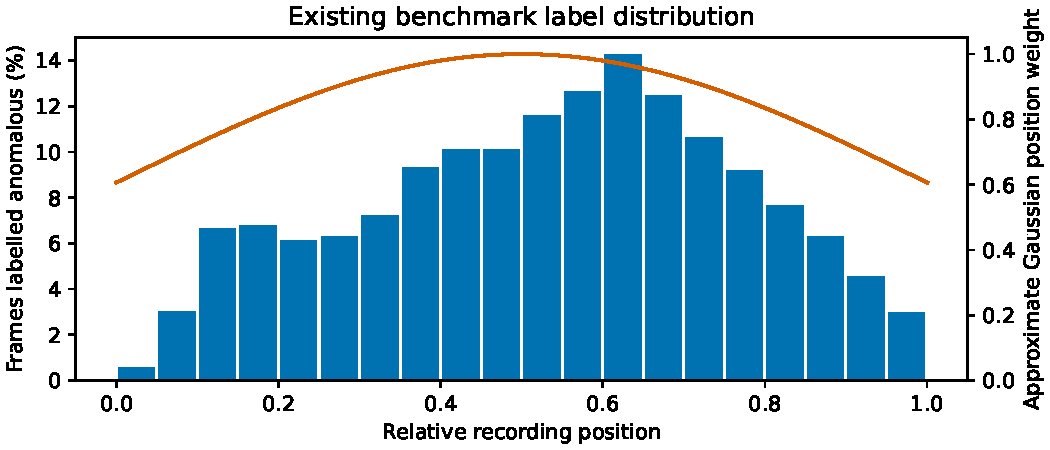
\includegraphics[width=.85\linewidth]{figures/label_positions.pdf}
\caption{Existing label distribution by relative recording position, with the approximate Gaussian weighting profile on the right axis. This is a benchmark annotation distribution, not a universal prior about when anomalies occur.}
\end{figure}

\section{Frozen protocol, corrections and reproducibility}
Protocol commit819ba57 preceded feature download; implementation and verified-asset freeze3da8543 preceded performance. The first launch stopped before reference execution because a relative evidence path became invalid after entering a temporary directory. Commitbc7e03f preserves its traceback and documents absolute CLI paths; frozen code was unchanged.

The second launch completed the upstream reference but independent replay failed for a 14-segment video: NumPy convolution returns 15 values when the kernel is longer, while upstream's loop reads only the first$N$. Amendment3cce2c8 truncates to$N$, exactly matching upstream. The failed attempt remains preserved. No offsets, input choices, criteria or bootstrap settings changed. All shift statistics used the successful third reconstruction. A new reference/replay cache avoided overwriting partial outputs.

Code, complete results, bootstraps, per-video/category diagnostics, input manifests and figures are versioned in the position-audit branch and PR12. Original PR11 prompt experiments are unchanged. External feature and raw-vector files are identified by hashes and reconstructed using the documented commands. No GPU fallback or automatic XD run is authorized by a statistical result.

\section{Novelty and limits}
VERA already ablates removal of position weighting (AppendixB.4/Table 17): \url{https://arxiv.org/html/2412.01095v2}. CoReVAD also ablates that operation (Table 4): \url{https://arxiv.org/html/2605.23116v1}. Removal is not a novel algorithm. The candidate contribution is controlled practical robustness measurement; the limited search not finding an identical replay study does not establish priority.

This experiment tests the final score multiplier, not edited-video inference, changed VLM sampling, scene transitions, streaming behavior or explanation truth. Benchmark labels remain imperfect and are not exhaustive semantic annotations. Independent XD/fresh confirmation and a broader novelty review would be needed for a general claim. No GPU experiment or learned extension is justified by this gate. Preserve the measurable finding and negative decision; do not lower the threshold or choose a sensitivity result post hoc.
\end{document}
